\documentclass{article}
\usepackage[a4paper]{geometry}
\pagestyle{empty}
\newgeometry{margin=1cm}
\usepackage{style}
\usepackage{graphicx}
\usepackage{ragged2e}
\usepackage{hyperref}
\usepackage{tikz}
\tikzstyle{dot}=[circle,fill,inner sep=2pt]

\makeatletter
\newcommand{\rubric}[1]{
    \centering
    \vspace{1cm}
    \section*{#1}
    \hrule
    \vspace{0.3cm}
    \raggedright
}

\begin{document}

\noindent
\begin{minipage}{0.3\textwidth}
  \includegraphics[width=\textwidth]{arnaud-cv}
\end{minipage}
\hfill
\begin{minipage}{0.6\textwidth}
  \noindent
  \centering
  \Huge \bfseries \texttt{ARNAUD PANNATIER}
  \vspace{4mm}

  \begin{minipage}{0.4\textwidth}
    \small \normalfont \noindent
    Rue des Longs-Prés 40 \\
    3960 Sierre \\
    VS, Switzerland \\
  \end{minipage}
  \hfill
  \begin{minipage}{0.4\textwidth}
    \small \normalfont
    \noindent Born 20 September 1995 \\
    Married \\
    Two children (2022,2023) \\
  \end{minipage}

  \small \normalfont \noindent
  \href{mailto:arnaud.pannatier@idiap.ch}{arnaud.pannatier@idiap.ch}\\
  \href{https://arnaudpannatier.ch}{https://arnaudpannatier.ch}\\
\end{minipage}

\vspace{1cm}
\hrule
\vspace{1cm}
\noindent I am a Ph.D. Student in François Fleuret's Machine Learning group (Idiap/EPFL). My main research interest are deep learning architectures and their applications on High-Altitude Wind Nowcasting. \\

\hspace{0.02\textwidth}
\begin{minipage}[t][0.98\textheight][t]{0.61\textwidth}
  \rubric{Education}
  \small
  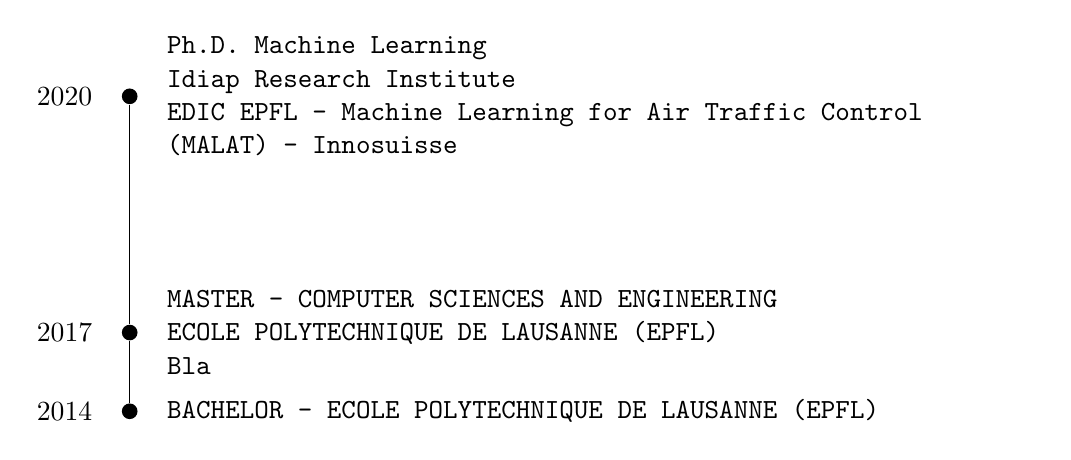
\begin{tikzpicture}
    \node[dot] (2020) at (0,4) {};
    \node[dot] (2017) at (0,1) {};
    \node[dot] (2014) at (0,0) {};
    \draw (2020)node[left=10pt] {2020};
    \draw (2020)node[right=10pt, text justified,text width=11cm] {\texttt{Ph.D. Machine Learning \\
        Idiap Research Institute \\
        EDIC  EPFL - Machine Learning for Air Traffic Control (MALAT) - Innosuisse}};
    \draw (2017)node[left=10pt] {2017};
    \draw (2017)node[right=10pt, text justified,text width=11cm]
    {\texttt{MASTER -  COMPUTER SCIENCES AND ENGINEERING \\
        ECOLE POLYTECHNIQUE DE LAUSANNE (EPFL) \\
        Bla
      }};
    \draw (2014)node[left=10pt] {2014};
    \draw (2014)node[right=10pt] {\texttt{BACHELOR - ECOLE POLYTECHNIQUE DE LAUSANNE (EPFL)}};
    \draw (2014) -- (2017) -- (2020);
  \end{tikzpicture}

  \rubric{Publications}

  Test test

  \rubric{Skills}

  \rubric{Languages}

  \rubric{Hobbies \& Interest}

\end{minipage}

\end{document}